\chapter{Background}
\label{chap:background}

This chapter provides a short introduction to ultrasound imaging in general and its use in the medical domain in particular. It then moves on to basic explanations on wave propagation, before moving deeper into the concept of \textit{beamforming}.
The excellent book 'Array Signal Processing - Concept and Techniques' by \cite{Dudgeon_book} has been a valuable source of information for this chapter.

Once the concept of conventional beamforming is thoroughly explained, this chapter builds on this theory to introduce the concept of \textit{adaptive beamforming} and presents different algorithms using that concept.
Most of the theory is first presented as broadly as possible, then narrowed down specifically to standard medical ultrasound imaging applications.


\section{Ultrasound imaging}
\label{sec:ultrasound_imaging}
Ultrasound imaging, also known as sonography or ultrasonography, is an imaging technique based on acoustic waves at frequencies above those audible by humans. It relies on the use of beamforming (Section \ref{sec:beamforming}) to give a spatial meaning to the recorded signals time and amplitude information. The frequency ranges used in ultrasound imaging vary depending on the application, but typically lie between $20~$kHz and $20~$MHz. This technology is used in multiple fields, some of the biggest being sonar (\cite{sonar}) and medical (\cite{medical_physics}).
Most ultrasound imaging systems can be classified into two groups:
\begin{itemize}
\item Passive: The system listens for sound waves emitted by sources in the zone of interest.
\item Active: The system emits sound waves and listen to echoes coming from the zone of interest.
\label{item:systems}
\end{itemize}

\subsection{Medical ultrasound imaging}
In the medical domain, ultrasound imaging is typically used as a noninvasive diagnostic tool to image body structures, such as organs or tissue. Ultrasound imaging systems are relatively cheap and portable, which makes them more accessible than the other imaging methods presented in Section \ref{sec:medical_imaging}.
Another advantage of ultrasound imaging is its ability to capture and process data in real-time, thus allowing real-time image analysis.
It is also considered safer than X-ray imaging, since it is based on non-ionizing radiation.
Besides its ability to image body elements, it can also be used to estimate blood flow velocities in arteries or vessels by analyzing the Doppler effect of backscattered signals (\cite{doppler_ultrasound}). The term 'Doppler ultrasound imaging' is then often used.

Since most, if not all, body structures do not emit acoustic waves, active imaging systems have to be used. A probe consisting of multiple transducers is typically pressed against the skin of the patient, and pointed towards the zone of interest, for example his/her heart, as illustrated in Figure \ref{fig:echocardiography}.

\begin{figure}[ht]
    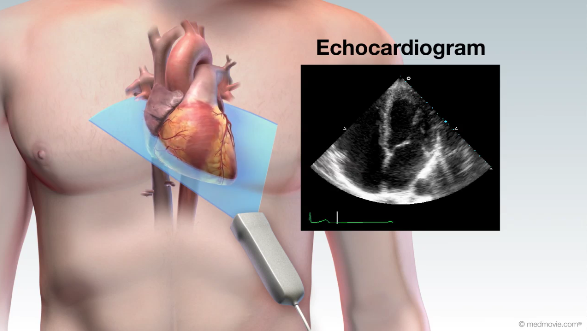
\includegraphics[width=\linewidth]{./images/background/echocardiogram.png}
	\caption{Illustration of ultrasound echocardiography (medmovie.com)}
	\label{fig:echocardiography}
\end{figure}

\subsection{Medical imaging}
\label{sec:medical_imaging}
Medical imaging refers to non-invasive techniques, unlike surgery, that provide a visual representation of internal body elements. Various imaging techniques exist, some of the most used ones being Magnetic Resonance Imaging (MRI), X-ray, Nuclear and Ultrasound. 
The choice of imaging technique depends on the the body part of interest and the diagnostic purpose. Table \ref{table:medical_imaging} shows a non-exhaustive comparison of those methods.

\begin{table}[!ht]
\centering
\begin{tabular}{| c || c |}
 \hline\hline
    &   Spatial resolution [mm] \\
  \hline
  Ultrasound    &   1 - 5 \\
  X-Rays    &   0.1 \\
  MRI   &   0.3 - 1 \\
  Nuclear   &   5 - 15 \\
  
  \hline\hline
    &   Safety \\
  \hline
  Ultrasound    &   No known hazards \\
  X-Rays    &   Small radiation dose \\
  MRI   &   Pacemakers and implants can be a hazard \\
  Nuclear   &   Moderate radiation dose \\
  
  \hline\hline
    &   Bone imaging \\
  \hline
  Ultrasound    &  Poor - Ultrasound does not penetrate bone \\
  X-Rays    &   Preferred technique \\
  MRI   &   Gives weak MRI signal \\
  Nuclear   &   Good for early diagnosis \\
  
  \hline\hline
    &   Heart and circulation imaging \\
  \hline
  Ultrasound    &  Preferred technique \\
  X-Rays    &   Needs contrast medium \\
  MRI   &    Good resolution capabilities \\
  Nuclear   &   Useful for flow studies \\
  \hline\hline
  
    &   Soft tissues imaging    \\
  \hline
  Ultrasound    & Preferred technique for areas with low bone density \\
  X-Ray &   Poor \\
  MRI   &   Preferred technique for muscles and joints \\
  Nuclear   & Poor \\
  \hline\hline
  
    &   Chest imaging   \\
  \hline
  Ultrasound    & Poor - Ultrasound can not image past air spaces \\
  X-Ray & Preferred technique for lung screening \\
  MRI   & Not good for imaging air spaces \\
  Nuclear   & Very good for air and blood flow imaging \\
  
  \hline\hline
  
    &   Brain and spinal cord imaging   \\
  \hline
  Ultrasound  & Poor - Difficult to image through skull \\
  X-Ray & Limited use \\
  MRI   & Preferred technique \\
  Nuclear   & Poor \\
  \hline
 \end{tabular}
\caption{Comparison of some of the main medical imaging techniques taken from 'Medical Physics: Imaging' by \cite{medical_physics}}
\label{table:medical_imaging}
\end{table}

\subsection{Therapeutic medical ultrasound}
Ultrasound is most widely used in the medical domain as a noninvasive diagnostic tool. It can however also be used for therapeutic applications. Ultrasound waves have been proven to cause local heating of tissue and increase in blood flow if radiating high levels of energy. It can also produce cavitation in extreme cases.
Ultrasound probes used for medical imaging are subject to strict restrictions in order to avoid or limit such effects. The use of such probes are therefore most of the time painless and completely harmless to the patient.

The potential side-effects of the use of ultrasound have however shown to be useful when used wisely. They gave birth to several therapeutic applications of ultrasound, such as targeted ultrasound delivery, high intensity focused ultrasound or lithotripsy, which is a procedure that uses shock waves to break up stones in the kidney, bladder, or ureter (\cite{lithotripsy}).

\section{Signal propagation and acquisition}
\label{sec:signals}

\subsection{Acoustic waves}
\label{sec:physics_waves}
A wave is an oscillation transferring energy in space without, or with little, transfer of mass. There are two main types of waves: \textit{Mechanical}, which can only propagate in a medium, and \textit{Electromagnetic}, which can propagate in vacuums as well.
\par
Ultrasound waves, and acoustic waves in general, are mechanical waves.
There exist two basic types of wave motion for mechanical waves: \textit{Longitudinal} and \textit{Transverse}. As shown in Figure \ref{fig:wave_types}, a longitudinal wave (P-wave) propagates through compression and dilatation along its direction of propagation, whereas a transverse wave (S-wave) propagates through oscillation of particles orthogonal of its direction of propagation.
In ultrasound medical imaging, the probe's transducers are oscillated in order to create pressure variations, and therefore longitudinal waves, in the imaged medium.
It is worth mentioning that transverse waves may be induced in that process and can be used in specific domains such as elastography.
However, in conventional ultrasound medical imaging, transverse waves are often ignored and therefore fall out of the scope of this thesis.

\begin{figure}[ht]
    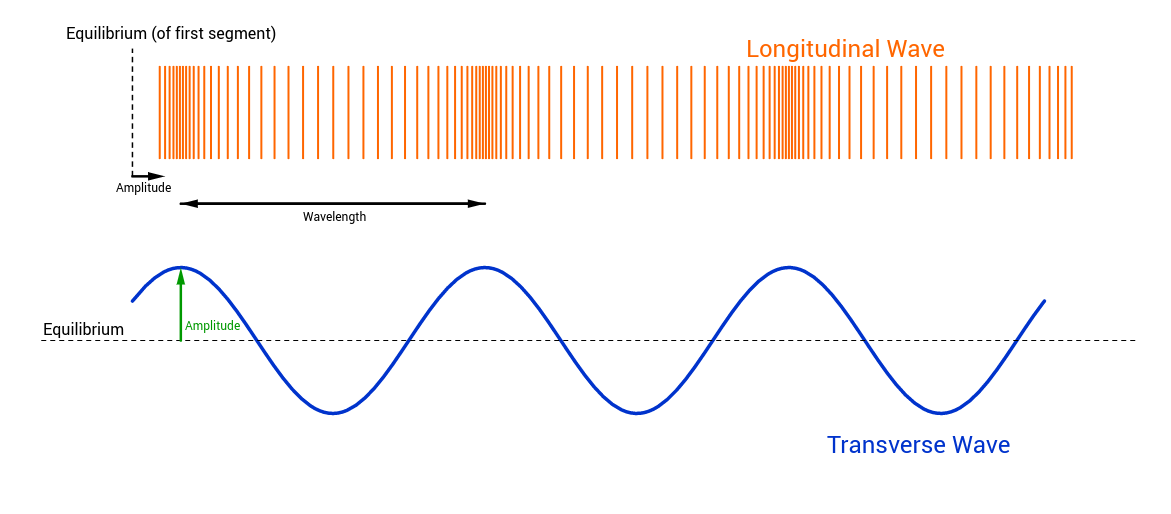
\includegraphics[width=\linewidth]{./images/background/wave_propagation.png}
	\caption{Longitudinal and transverse waves propagation. Illustration generated with \cite{wave_propagation}}
	\label{fig:wave_types}
\end{figure}


\subsection{Propagating waves}
\label{sec:prop_waves}
Information can be transmitted from one transducer to another by the means of propagating waves. The actual physics of the propagation depends on the type and properties of the wave and of the medium in which it propagates. Luckily a single formula can be used both for electromagnetic waves and acoustic waves. The lossless wave equation describes the propagation of a waveform $s(\boldsymbol{x}, t)$ in an ideal medium:
\begin{equation}
    \nabla^2 \boldsymbol{s} = \frac{\delta^2 \boldsymbol{s}}{\delta x^2} + \frac{\delta^2 \boldsymbol{s}}{\delta y^2} + \frac{\delta^2 \boldsymbol{s}}{\delta z^2} = \frac{1}{c^2} \frac{\delta^2 \boldsymbol{s}}{\delta t^2},
\end{equation}
\noindent
where $\boldsymbol{x} = (x, y, z)$ is the three dimensional spatial variable, $t$ the time variable, $\nabla^2$ is the Laplacian operator and $c$ the wave's speed of propagation. An ideal medium is a medium that does not induce any disturbance to the propagation of the wave, such as dispersion, refraction or attenuation. The lossless wave equation can easily be derived from Maxwell's equations for electromagnetic waves. For acoustic waves, the same equation can be built from fundamental physics principles (conservation of mass, equation of state, Newton's second law of motion). The derivation of the wave equation is however much more complicated for acoustic wave due to the fact that there is no unified set of equations, such a Maxwell's equations, defining all acoustic waves. The proof of the lossless wave equation is not provided in this thesis.

For electromagnetic waves, $c = \sqrt{\epsilon \mu}$, where $\epsilon$ is the medium's dielectric permittivity and $\mu$ is its magnetic permeability. For acoustic waves, $c$ is dependent on the medium's pressure and density.
As a rule of thumb, electromagnetic waves typically propagate at speeds in the order of $10^8 ~ m/s$  ($3 \cdot 10^8$ in free space) whereas acoustic waves propagate much slower, typically in the order of hundreds or thousands of m/s.

A monochromatic wave is a wave composed of a single frequency $\omega$. Such a wave can be described in the time domain as a complex exponential of frequency $\omega$:
\begin{equation}
    s(\boldsymbol{x},t) = A e^{j \omega t + \phi},
\label{eq:mono_wave}
\end{equation}
\noindent
where $A$ is a real or complex valued amplitude factor and $\phi$ is a phase delay dependent on $\boldsymbol{x}$.
Assuming that $\phi = 0$ at $x_0 = (0, 0, 0)$ and $\boldsymbol{x}$ is at distance $D = |\boldsymbol{x}|$ from $x_0$, the phase delay $\phi$ is then $\phi = \omega D / c$, where $c$ is the wave's speed of propagation

The theory presented in this section focuses on monochromatic waves, but Equation (\ref{eq:mono_wave}) can be extended to nonmonochromatic waves by applying the superposition principle:
\begin{equation}
    s(\boldsymbol{x},t) = \sum_{i=1}^I A_i e^{j \omega_i t + \phi_i},
\label{eq:superpos}
\end{equation}
\noindent
where $I$ is the length of the set $\Omega = [\omega_1, ..., \omega_I]$ of frequencies present in $s(\boldsymbol{x},t)$.
In practice, $\Omega$ is often an infinite set and Equation (\ref{eq:superpos}) is approximated with a finite set of frequencies.

Although waves are fundamentally considered as \textit{spherical} waves, they can sometimes be approximated to \textit{plane} waves.
Whereas spherical waves propagate in all directions, a plane wave can be seen as propagating in a single direction $\boldsymbol{\zeta}$.
Its phase delay can then be defined as $\phi = \omega \boldsymbol{\zeta} \cdot \boldsymbol{x} / c$.
The wave's propagation speed $c$ and direction $\boldsymbol{\zeta}$ are often combined into the wave's slowness vector $\boldsymbol{\alpha} = \boldsymbol{\zeta} / c$.
The equation of a monochromatic plane wave can then be expressed as a function of a single variable:
\begin{equation}
    s(\boldsymbol{x},t) = A e^{j \omega ( t - \boldsymbol{\alpha} \cdot \boldsymbol{x})} = s(t - \boldsymbol{\alpha} \cdot \boldsymbol{x}).
\label{eq:mono_plane_wave}
\end{equation}
\noindent
The same equation is also often written as $s(\boldsymbol{x},t) = A e^{j (\omega t - \boldsymbol{k} \cdot \boldsymbol{x})}$, where $\boldsymbol{k} = \omega \boldsymbol{\alpha}$ is the wave's wavenumber vector.
The wavenumber vector is a vector whose direction follows the direction of propagation $\boldsymbol{\zeta}$ and whose magnitude $|\boldsymbol{k}| = \omega / c$ represents the number of cycles (of temporal period $T = 2\pi / \omega$) per meter the monochromatic wave exhibits along that direction. The inverse relation, i.e. the distance propagated during one period $T$, is the wave's \textit{wavelength} $\lambda = 2\pi / |\boldsymbol{k}|$.

The term \textit{plane wave} is used because any point lying in the plane $k_x x + k_y y + k_z z = C$, where $C$ is a constant, experiences the same value of $s(\boldsymbol{x},t)$.
This plane wave approximation is used in farfield beamforming (Section \ref{sec:nearfield_farfield}).

Real media often diverge from the ideal medium in the fact that they can induce disturbances to propagating waves, such as dispersion, attenuation or refraction to name only a few. Such disturbances are numerous, complex and still studied to this day. Since the physics of wave propagation is not the focus of this thesis, those divergences are not further explored. The 'Array Signal Processing - Concept and Technique' book by \cite{Dudgeon_book} provides more thorough explanations on the topic.


\subsection{Signal transmission and recording}
\label{sec:sensor_arrays}
In order to represent physical waves by an electrical signal (i.e. recording), a transducer able to convert propagating energy into electrical energy must be designed. The same holds for signal transmission, converting electrical energy into propagating energy.
Transducers can be designed for either or both of these functions.
An \textit{omnidirectional} transducer simply samples the field at a particular location and/or transmits a spherical wave, propagating in all directions at the same speed, if in the same medium. Note that a transducer would have to be infinitely small to be able to transmit truly spherical waves. A \textit{directional} transducer has the ability to focus its signal recording and/or transmission on a particular propagation direction.

The equation of a spatiotemporal signal is, as its name indicates, a function of space and time $f(\boldsymbol{x}, t)$, where $\boldsymbol{x} = (x, y, z)$ is the three dimensional spatial variable and $t$ the time variable. A single transducer at location $\boldsymbol{x}_m$ can convert the field's value at its location $f(\boldsymbol{x}_m, t)$ and output a corresponding electrical signal $y_m(t)$. Due to the transducer's finite bandwidth and non-linear transformation, $y_m(t)$ most of the time does not fully represent $f(\boldsymbol{x}_m, t)$ and some information is lost during the energy conversion.

Real transducers are not truly infinitely small, so their position is not restrained to a single point $\boldsymbol{x}_m$. A transducer's \textit{aperture} can be represented by the set of positions $\boldsymbol{X}_m$ for which it can gather signal energy. Its \textit{aperture function}, in its simplest form, describes its aperture geometry:
\begin{equation}
    w(\boldsymbol{x}) = \left \{ \begin{tabular}{cc}
        1, & $\boldsymbol{x} \in \boldsymbol{X}_m$ \\
        0, & otherwise
    \end{tabular}\right..
\end{equation}
\noindent
As example, let us consider a transducer as a linear surface of length $D$ along the X axis such that $\boldsymbol{x}_m = (0, 0, 0)$ is a the center of the transducer. Such a transducer can be described by the following aperture function:
\begin{equation}
    w(\boldsymbol{x}) = \left \{ \begin{tabular}{cc}
        1, & x $\leq$ D/2, ~ y = 0, ~ z = 0 \\
        0, & otherwise
    \end{tabular}\right.,
\label{eq:aperture_linear}
\end{equation}
\noindent
where $x$, $y$ and $z$ are the 3D components of the position vector $\boldsymbol{x}$.

Besides defining the transducer geometry, the aperture function can also define the relative weighting of the field within the aperture. This concept of aperture weighting, also known as shading, tapering or apodization, is actively used in adaptive beamforming methods (Section \ref{sec:adaptive_beamforming}).


\subsection{Aperture smoothing function}
\label{sec:aperture_smoothing}
In most, if not all, signal processing applications, it is often useful to have a frequency-domain representation of signals. Among other advantages, it makes it easy to analyze the frequency content of any signal and intuitive to represent any signal by a weighted sum of sinusoidal functions. The Fourier Transform and its inverse function are very useful tools to alternate between time-domain and frequency-domain representations. The Fourier Transform of a spatiotemporal signal $s(\boldsymbol{x},t)$ can be written as:
\begin{equation}
    S(\boldsymbol{k}, \omega) = \int_{-\infty}^{\infty} \int_{\mathbb{R}^3} s(\boldsymbol{x},t) e^{-j(\omega t - \boldsymbol{k} \cdot \boldsymbol{x})} d\boldsymbol{x} dt,
\end{equation}
\noindent
where $\boldsymbol{k}$ is the signal's wavenumber vector variable and $\omega$ its frequency variable. A transducer \textit{aperture smoothing function $W(\boldsymbol{k})$} is defined as the Fourier Transform of its aperture function $w(\boldsymbol{x})$.

Going back to the example of Section \ref{sec:sensor_arrays}, Equation (\ref{eq:aperture_smoothing_linear}) develops how the transducer's aperture smoothing function is calculated from its aperture function defined in Equation (\ref{eq:aperture_linear}). Figure \ref{fig:linarray} illustrates how such an transducer and aperture smoothing function look.
\begin{align}
    W(\boldsymbol{k}) &= \int_{\mathbb{R}^3} w(\boldsymbol{x}) e^{j \boldsymbol{k} \cdot \boldsymbol{x}} d\boldsymbol{x} = \int_{-D/2}^{D/2} e^{j k_x x} dx \nonumber \\
    &= \frac{1}{j k_x} (e^{j k_x D/2} - e^{-j k_x D/2}) \nonumber \\
    &= \frac{2j}{2k_x} (e^{-j k_x D/2} - e^{j k_x D/2}) \nonumber \\
    &= \frac{\sin(k_x D/2)}{k_x/2}.
\label{eq:aperture_smoothing_linear}
\end{align}

\begin{figure}[ht]
    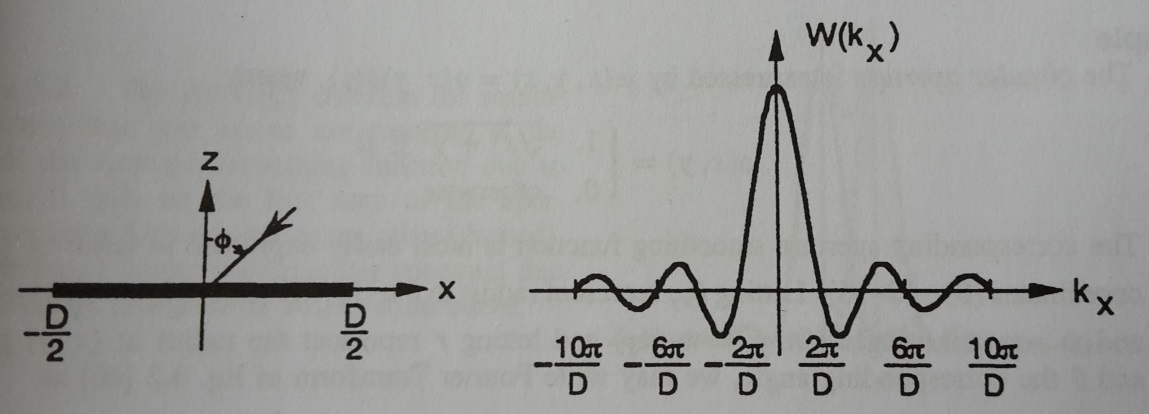
\includegraphics[width=\linewidth]{./images/background/linarray.jpg}
	\caption{Illustration of a linear array and its aperture smoothing function (Johnson and Dudgeon 1993, p.115)}
	\label{fig:linarray}
\end{figure}
\noindent
The transducer aperture smoothing function has a shape similar to a sinc function, with a mainlobe at $k_x = 0$ and sidelobes decreasing in amplitude as $k_x$ increases towards $\infty$ or decreases towards $-\infty$. Equation (\ref{eq:aperture_smoothing_linear}) also reveals that the longer the transducer is, the narrower the aperture smoothing function's mainlobe is. A narrow mainlobe is often a desired feature in beamforming, as it can increase the \textit{angular resolution} of the resulting image. There exists many definitions of \textit{resolution} in ultrasound imaging, which is why it may be confusing to compare results from different articles.

In this thesis, angular resolution is defined as the minimum distance between two reflectors for them to be resolved. This measure, often referred to as \textit{classical resolution} or \textit{resolvability}, is governed by the Rayleigh criterion. The Rayleigh criterion states that two incoherent plane waves propagating in different directions can be resolved if the distance between the mainlobe of their resulting aperture smoothing function replica is not smaller than half of the largest mainlobe width.

Notice however that the Rayleigh criterion only defines a theoretical maximum resolution and not an actual resolution measurement. Also, for this definition to make sense, one must define how mainlobe width is measured. Figure \ref{fig:linarray} shows that this width differs depending on the gain level. In this thesis, a mainlobe width is always measured at -3 dB gain from its peak. On the same note, two waves are considered \textit{resolved} only if the minima between their peaks is less or equal than the lowest peak gain minus 3 dB.

\subsection{Transducer arrays}
\label{sec:discrete_arrays}
A single transducer, even directional, can not give accurate spatial meaning to a recorded wavefield, since it only outputs an electrical signal $y_m(t)$ as a function of time.
The concept of \textit{beamforming} (Section \ref{sec:beamforming}) uses the combined output of multiple transducers to give spatial meaning to a recorded wavefield.
Such a combination of transducers is called a transducer \textit{array}. A transducer array can be of virtually any shape, for example circular, spherical or sparse.  The aperture function $w_m(\boldsymbol{x})$ of each transducer is defined by Equation (\ref{eq:aperture_linear}), but the array itself can also be considered to have an aperture shape $w_a(\boldsymbol{x})$, regardless of the shape of each transducer:
\begin{equation}
    w_a(\boldsymbol{x}) = \left \{ \begin{tabular}{cc}
        1, & x $\in \boldsymbol{X}_a$ \\
        0, & otherwise
    \end{tabular}\right.,
\label{eq:aperture_global}
\end{equation}
\noindent
where $\boldsymbol{X}_a$ is the set of positions $\boldsymbol{x}_m$ of the array elements.

Despite the theory presented being applicable to various array shapes, this thesis only focuses on discrete linear arrays of transducers able to both transmit and record signals, since it is the type of array simulated in this thesis and still one of the most widely used types of array in medical ultrasound.

Let us then assume a discrete linear array consisting of M infinitely small transducers uniformly distributed along the X axis, each separated by a distance D. Let us also consider that $x = 0$ is the center of the array. For simplicity, let us further assume that M is odd, so that the transducers can be numbered from $m = -(M-1)/2$ to $m = (M-1)/2$ and their position can be expressed simply as $x = m D$.
The array aperture function is then:
\begin{equation}
    w_a(\boldsymbol{x}) = \left \{ \begin{tabular}{cc}
        1, & x = m D, ~ y = 0, ~ z = 0 \\
        0, & otherwise
    \end{tabular}\right..
\label{eq:array_aperture}
\end{equation}
\noindent
The array aperture smoothing function, defined as the Fourier Transform of Equation (\ref{eq:array_aperture}), is:
\begin{align}
    W_a(\boldsymbol{k}) &= \int_{-\infty}^{\infty} w(\boldsymbol{x}) e^{j \boldsymbol{k} \cdot \boldsymbol{x}} d\boldsymbol{x} = \sum_{m=-(M-1)/2}^{(M-1)/2} e^{j k_x D m} \nonumber \\
    &= e^{-j k_x D (M-1)/2} k\sum_{m=0}^{M-1} e^{j k_x D m} \nonumber \\
    &= e^{-j k_x D M/2} e^{j k_x D/2} \frac{1 - e^{j k_x D M}}{1 - e^{j k_x D}} \nonumber \\
    &= \frac{2j}{2j} \frac{e^{-j k_x D M/2} - e^{j k_x D M/2}}{e^{-j k_x D/2} - e^{j k_x D/2}} \nonumber \\
    &= \frac{\sin(k_x D M/2)}{\sin(k_x D/2)},
\label{eq:array_aperture_smoothing}
\end{align}
\noindent
where the lemma $\sum_{n=0}^{N-1} r^n = \frac{1 - r^N}{1 - r}$ has been used.
\par
Equation (\ref{eq:array_aperture_smoothing}) reveals that the array smoothing function, unlike that of a single transducer (Equation (\ref{eq:aperture_smoothing_linear})), is periodic. This function is maximized for $k_x = n 2\pi/D, n \in \mathbb{Z}$, only one of which is the mainlobe ($k_x = 0$). The other maximas are called \textit{grating lobes}. This can result in \textit{spatial aliasing}, as signals propagating from different directions become indistinguishable.
However the array elements' own aperture geometry influence the array's total aperture $w_t(\boldsymbol{x})$.
The array aperture smoothing function of a discrete linear array can be defined as the product of a single element aperture smoothing function $W_m(\boldsymbol{k})$ and the one of the same array with infinitely small elements $W_a(\boldsymbol{k})$ (\cite{knut_landmark}):
\begin{equation}
    W_t(\boldsymbol{k}) \equiv W_m(\boldsymbol{k}) \cdot W_a(\boldsymbol{k}).
\end{equation}
\noindent
Figure \ref{fig:total_aperture} illustrates the effect of a transducer's aperture smoothing function applied to the one of the array. $W_m(\boldsymbol{k})$ is a non-periodic function, so the resulting effect is an attenuation of the array aperture smoothing function in all directions $\boldsymbol{k}$ with $k_x \neq 0$. One positive outcome of this attenuation is that the resulting function $W_t(\boldsymbol{k})$ has attenuated side lobes and grating lobes and is therefore less prone to signal propagation confusion.


\begin{figure}[ht]
    \centering
    \begin{subfigure}[b]{0.48\linewidth}
        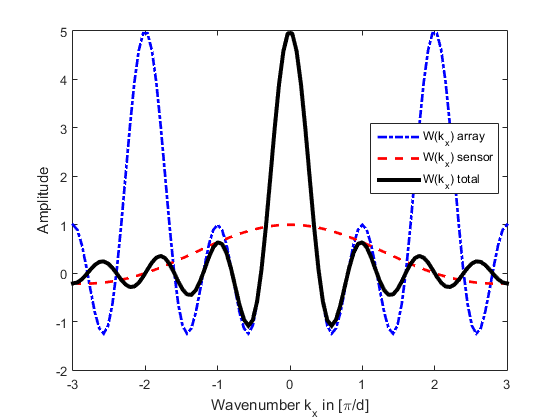
\includegraphics[width=\linewidth]{./images/background/bg_grating1.png}
        \caption{$W(k_x)$ amplitude}
    \end{subfigure}
    \quad
    \begin{subfigure}[b]{0.48\linewidth}
        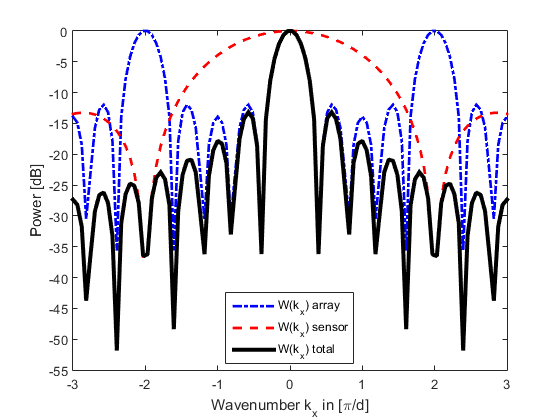
\includegraphics[width=\linewidth]{./images/background/bg_grating2.png}
        \caption{$W(k_x)$ power}
    \end{subfigure}
	\caption{Aperture smoothing function of discrete linear array of M=5 transducers}
	\label{fig:total_aperture}
\end{figure}


\section{Conventional beamforming}
\label{sec:beamforming}
Beamforming is a signal processing technique using multiple transducers to restrain the directionality of signals transmission or reception (\cite{DAS}). In the case of near-field beamforming (Section \ref{sec:nearfield_farfield}), this technique also restrains the range of focus. Medical ultrasound imaging is an example of a near-field scenario. And, since it uses active systems (Section \ref{sec:medical_imaging}), the beamforming can be done both on transmission and reception. This is often referred as \textit{two-way beamforming}, while \textit{one-way beamforming} designates beamforming on reception only. Although based on the same theory, beamforming on transmission and reception have two different goals:
\begin{itemize}
    \item Transmission: Produce signals such that they become all in phase at the focus point and result in a maximized energy radiation towards it.
    \item Reception: Align the recorded signals such that any potential signal coming from the focus point adds up coherently and maximizes its signal-to-noise ratio (SNR) when all recorded waveforms are summed together. The same approach can be applied to different focus points on the same signal measurements, which is why it is often referred to as \textit{dynamic focusing}.
\end{itemize}
\noindent
In this thesis, all beamformers use two-way beamforming and create beamformed images by sequentially transmitting narrow beams in a number of directions and, for each transmitted beam, dynamically delaying the received signals from all channels.

\subsection{Beamforming on transmission}
\label{sec:beamforming_transmission}
Whenever multiple waves are present in a wavefield, their superposition may result in interference.
As an example, let us imagine two monochromatic plane waves $s_1(\boldsymbol{x}, t)$ and $s_2(\boldsymbol{x}, t)$ of same frequency $\omega$ and amplitude $A$ being transmitted by two different emitters $t_1$ and $t_2$. The equation of such waves can be extracted from Equation (\ref{eq:mono_plane_wave}):
\begin{equation}
    s_i(x, t) = A ~ e^{j (\omega t - \boldsymbol{k}_i \cdot \boldsymbol{x} + \Phi_i)}, ~ i = [1, 2],
\end{equation}
\noindent
where $\Phi_i$ is the phase value of $s_i$ at position $\boldsymbol{x} = (0, 0, 0)$.
Let us have a receiver $r$ exposed to those waves. Its wavefield measurement $y_r(\boldsymbol{x}_r, t)$ is then, according to the superposition principle, equal to the sum of the two waves at that location and time:
\begin{align}
    y_r(\boldsymbol{x}_r, t) &= s_1(\boldsymbol{x}_r, t) + s_2(\boldsymbol{x}_r, t) \nonumber \\
    &= A ~ e^{j \omega t} (e^{-j (\boldsymbol{k}_1 \cdot \boldsymbol{x}_r - \Phi_1)} + e^{-j (\boldsymbol{k}_2 \cdot \boldsymbol{x}_r - \Phi_2)}),
\end{align}
\noindent
where $e^{-j (\boldsymbol{k}_1 \cdot \boldsymbol{x}_r - \Phi_1)} + e^{-j (\boldsymbol{k}_2 \cdot \boldsymbol{x}_r - \Phi_2)}$ is a periodic function with values in the [-2, 2] range, which means that, depending on the receiver's position $\boldsymbol{x}_r$, it can be exposed to energy amplitudes ranging from 0 to 2A. The waves interference is often referred to as \textit{constructive interference} when the recorded energy amplitude is higher than A, respectively \textit{destructive interference} when lower amplitude than A.

The example above shows that the effects of constructive interference can be used to achieve higher SNR than when transmitting a single signal.
Beamforming on transmission uses this physical property to aim towards a spatial point $\boldsymbol{x}_t$ and ensure constructive interference of its transmitted signals in that point.

Given an array of M transducers, each sending a signal $s_m(t) = s(t - \Delta_m)$, the delays $\Delta_m$ can be made such that constructive interference occurs at the focus point $\boldsymbol{x}_t$. The set of those time-based delays $\boldsymbol{e} = [\Delta_0, \Delta_1, ..., \Delta_{M-1}]^T$ can be seen as a beamforming focus vector, since it defines at which positions $\boldsymbol{x}$ constructive, and respectively destructive, interference occurs.


\subsection{Beamforming on reception}
\label{sec:beamforming_reception}
Given an array of M transducers and a set $Y(t) = [y_1(t), y_2(t), ..., y_M(t)]^T$, where $y_m(t)$ is the data recorded by transducer $m$.

Beamforming on reception can be done in a similar way as beamforming on transmission by creating a set of time-delays $\boldsymbol{e} = [\Delta_1, ..., \Delta_M]^T$ and applying the time-delays to the recorded data. Given any receive focus point $\boldsymbol{x}_r$, the time-delays set $\boldsymbol{e}_r$ is built such that any potential signal coming from $\boldsymbol{x}_r$ gets aligned coherently in the recorded data $Y(t)$.
Let us define the set of time-delayed recorded data $Y_e(t) = [y_{1e}(t), y_{2e}(t), ..., y_{Me}(t)]^T$, where $y_{me}(t) = y_m(t - \Delta_m)$.

Assuming a signal $s(t)$ sent towards the array from a source at position $\boldsymbol{x}_r$, each transducer's recorded wavefield $y_m(t)$ can be defined as:
\begin{equation}
    y_m(t) = s(t - \Delta_{rm}) + n_m(t),
\end{equation}
\noindent
where $\Delta_{rm}$ is a time delay attribute dependent on the position of transducer $m$ relative to the position of the source and the signal propagation properties, and $n_m(t)$ random noise recorded by transducer $m$.
The beamformer can focus on the source position by applying time delays equal to $-\Delta_{rm}$. Given $\boldsymbol{e}_r = [-\Delta_{r1}, -\Delta_{r2}, ..., -\Delta_{rM}]$, the time-delayed vectors $y_{me}(t)$ are then:
\begin{align}
    y_{me}(t) &= y_m(t - \Delta_m) = y_m(t + \Delta_{rm}) \nonumber \\
    &= s(t) + n_m(t + \Delta_{rm}).
\end{align}

The signal $s(t)$ can then be added constructively and result in a signal power $M$ times higher than if recorded by a single transducer. If the noise $n_m(t)$ recorded by each transducer is assumed to be white noise, it can be considered to be statistically uncorrelated to $n_i(t),~i \neq m$. This means that the sum of time-delayed signals also results in a signal SNR $M$ times higher than that of a single transducer recording.

Signals coming from other sources are expected to result in lower SNR than the one coming from $\boldsymbol{x}_r$, although, as seen in Section \ref{sec:aperture_smoothing}, this can not always be guaranteed.
The terms \textit{constructive} and \textit{destructive interference} are usually connoted to physical interference, so they are not used in this thesis for beamforming on reception to avoid confusion.


\subsection{Delay-And-Sum (DAS) beamforming}
\label{sec:DAS}
DAS beamforming is one of the simplest beamforming algorithms, yet still widely used in medical ultrasound imaging. The DAS beamformer's output signal can be defined as:
\begin{equation}
    z(t) \equiv \sum_{m=0}^{M-1} w_m y_m(t - \Delta_m),
\label{equ:das}
\end{equation}
\noindent
where $y_m(t - \Delta_m)$ is the data recorded by transducer $m$ after time-delay (Section \ref{sec:beamforming_reception}) and $w_m$ is the amplitude weight applied that data. If no shading (Section \ref{sec:sensor_arrays}) is applied, then $w_m = 1 \forall m \in \{0, 1, ..., M-1\}$. 
With the set of time-delayed received signals $\boldsymbol{Y}_e(t) = [y_{1e}(t), ..., y_{Me}(t)]^T$ defined as in Section \ref{sec:beamforming_reception}, Equation (\ref{equ:das}) can be rewritten in the vectorial form as:
\begin{equation}
    z(t) = \boldsymbol{w}^H \boldsymbol{Y_e}(t),
\end{equation}
\noindent
where $\boldsymbol{w}$ is the vector of amplitude weight values $w_m$ applied to transducer $m$ and $\boldsymbol{w}^H$ its conjugate transpose.

By using dynamic focusing on reception, a different time-based focus vector $\boldsymbol{e_x}$ can be defined for each focus point $\boldsymbol{x}$ in the imaged sector. 
The DAS beamformer output power can then be defined as a function of f $\boldsymbol{e_x}$:
\begin{equation}
\begin{split}
    Z(\boldsymbol{e_x}) \equiv E[|z(t)|^2](\boldsymbol{e_x}) = E\{(\boldsymbol{w}^H \boldsymbol{Y_{ex}})(\boldsymbol{w}^H \boldsymbol{Y_{ex}})^H\} \\
    = \boldsymbol{w}^H E\{\boldsymbol{Y_{ex}} \boldsymbol{Y_{ex}^H} \} \boldsymbol{w} = \boldsymbol{w}^H \boldsymbol{R_e} \boldsymbol{w},
\end{split}
\label{eq:das_power}
\end{equation}
\noindent
where $E[]$ is the expected value function and $\boldsymbol{R_e}$ is the \textit{spatial correlation matrix}, or \textit{covariance matrix}, of $\boldsymbol{Y_{ex}}$. Section \ref{sec:covariance_estimation} explains how this matrix can be estimated.

\subsection{Beamforming with narrowband signals}
\label{sec:beamforming_frequency}
Considering a monochromatic signal $s(t) = e^{j \omega t}$, a time-shift of $\Delta_m$ corresponds to a phase-shift of $e^{-j \omega \Delta_m}$:
\begin{equation}
    s(t - \Delta_m) = e^{j \omega (t - \Delta_m)} = e^{j \omega t} e^{-j \omega \Delta_m}.
\end{equation}
\noindent
Steering the transducers array can then easily be done by multiplying the set of received signals $Y_m(\omega)$ with a set of phase delays $e^{-i \omega \Delta_m}$. This set of phase-delays define the beamformer's phase-based \textit{steering vector} \textbf{a}.
Unlike the time-based focus vector \textbf{e} (Section \ref{sec:beamforming_transmission}), the phase-based one is only properly defined for a single frequency $\omega$. In fact, for any frequency $\omega_2 \neq \omega$, the phase shift $e^{-i \omega \Delta_m}$ differs of that of the $e^{-i \omega_2 \Delta_m}$ phase required for constructive signals superposition at the chosen focus point.

Although only valid for monochromatic waveforms, the phase-based steering approach is often used in narrowband applications, for which most of the energy radiated or recorded is within a small frequency bandwidth relative to the center frequency. In such scenarios, the phase shift difference $e^{-i (\omega_2 - \omega) \Delta_m}$ can be considered negligible.
In broadband applications, such as ultrasound medical imaging, the phase shift difference can only be considered negligible for small shifts, meaning for steering angles close to perpendicular to the array. For larger steering angles, the time-based dynamic focusing approach (Section \ref{sec:beamforming_reception}) can be used to fall back to reasonable phase shifts (\cite{Jensen_multibeam}). This technique is used throughout this thesis and all the theory presented from this point on is focusing on monochromatic waveforms.


\subsection{Near-field and far-field beamforming}
\label{sec:nearfield_farfield}
As mentioned in Section \ref{sec:prop_waves}, waves do not propagate along a single direction, but in all directions such that the set of coordinates with the same wave phase looks like a sphere, as illustrated in Figure \ref{fig:farfield}. Due to this type of propagation, sensors at different locations can experience a different wave propagation direction. This seems logical since the source of the propagating wave is potentially located at different relative orientations to each sensor. It is this difference in relative propagation direction that allows the possibility to focus a sensor array to a specific point in space.

However, if a wave's direction of propagation is approximately equal for all sensors, the perceived waveform resembles more the one of a plane wave, as illustrated in Figure \ref{fig:farfield}. This scenario can occur if the source of the propagating wave is located far from the array and plane wave approximation (Section \ref{sec:prop_waves}) can be applied. In that case, beamforming can resolve the source orientation but not its distance to the array.

Sources located close enough to the array to extract their distances to it are said to be in the array's \textit{near field}, whereas sources beyond that are said to be in its \textit{far field}. In most cases, the focus of interest is either in the near field or in the far field and different beamforming algorithms are usually used in either case. Therefore the terms \textit{nearfield beamforming} and \textit{farfield beamforming} are often used to differentiate the two scenarios.

The crossover distance $d_c$ between near field and far field is not a hard-defined one. It is based on deciding at which distance to the array the different wave propagation directions perceived by each sensor can be approximated to equal directions with a negligible phase error. The definition of negligible can vary a lot depending on the beamforming application and expected outcome.

An intuitive example of the crossover distance for linear arrays can be found in \cite{wright_compendium}. This example's crossover distance is $d_c = A^2 / \lambda$, where $A$ is the length of the linear array and $\lambda$ is the maximum signal wavelength present in the recorded wavefield.
In conventional ultrasound imaging, the array's length is typically in the order of centimeters, whereas the signals transmitted are in the order of $MHz$. Given the crossover distance $d_c = A^2 / \lambda$, most of the medical ultrasound imaging applications occur in the array's near field.

\begin{figure}[ht]
    \centering
    \begin{subfigure}[b]{0.48\linewidth}
        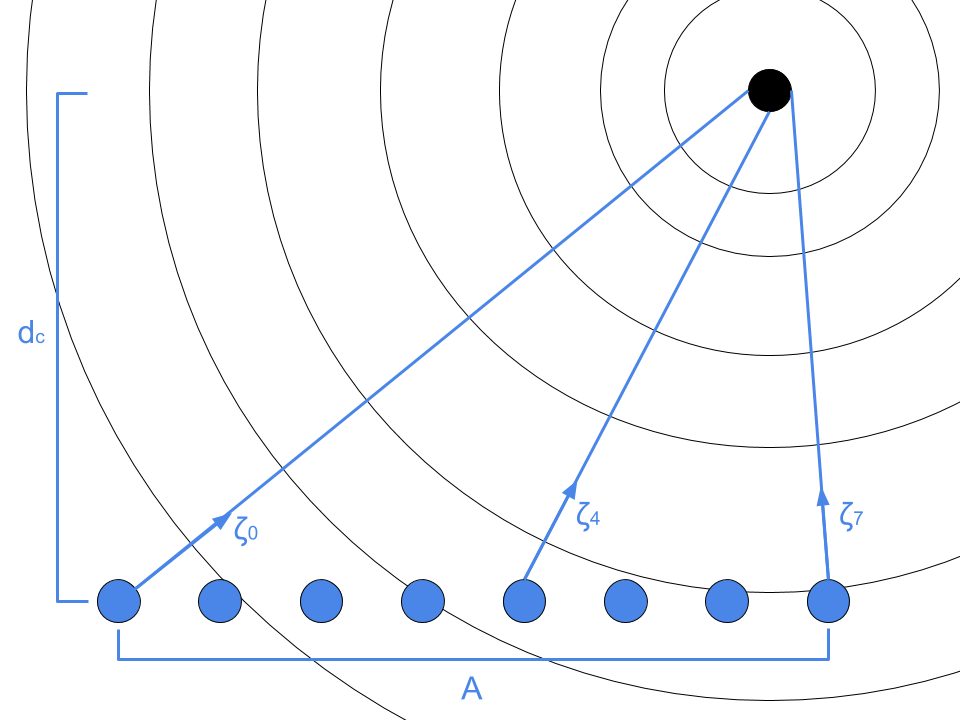
\includegraphics[width=\linewidth]{./images/background/nearfield.png}
        \caption{Nearfield}
    \end{subfigure}
    \quad
    \begin{subfigure}[b]{0.48\linewidth}
        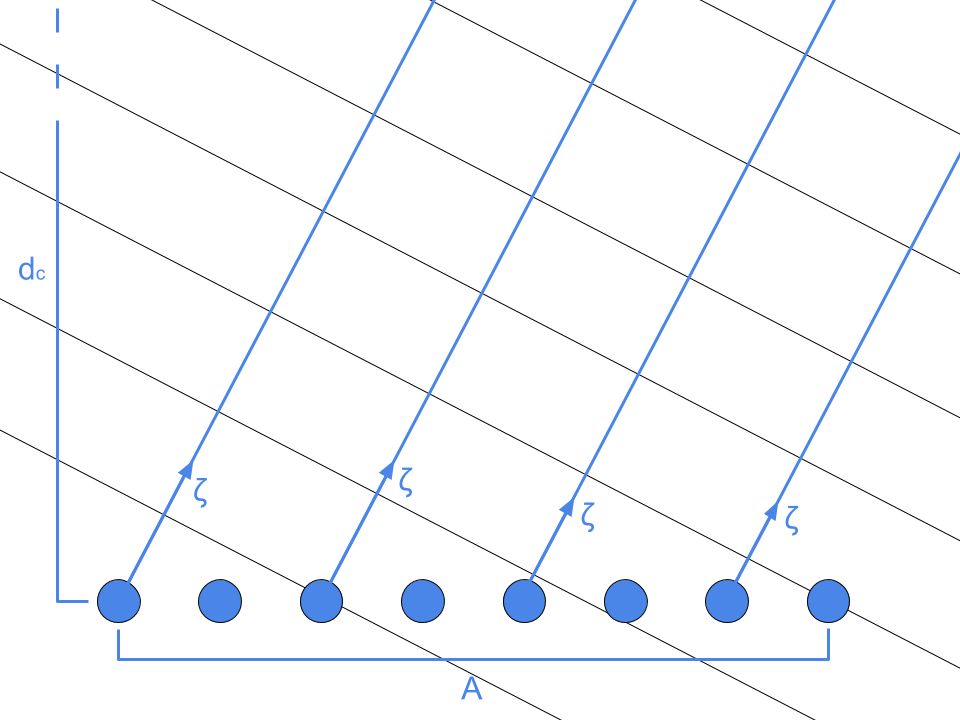
\includegraphics[width=\linewidth]{./images/background/farfield.png}
        \caption{Farfield}
    \end{subfigure}
	\caption{Illustrations of nearfield and farfield beamforming. The black lines and curves represent planes of constant phase.}
	\label{fig:farfield}
\end{figure}


\subsection{Beampattern and steered response}
\label{sec:beampattern} 
An array's aperture smoothing function, or array pattern, $W(\boldsymbol{k})$ defines its response to a monochromatic plane wave.
For a discrete array of M transducers, its aperture function $w(\boldsymbol{x})$ is defined by Equation (\ref{eq:aperture_global}) and its array pattern $W(\boldsymbol{k})$ from Equation (\ref{eq:array_aperture_smoothing}) as:
\begin{equation}
    W(\boldsymbol{k}) = \int_{\mathbb{R}^3} w(\boldsymbol{x}) e^{j \boldsymbol{k} \cdot \boldsymbol{x}} d\boldsymbol{x} = \sum_{m=0}^{M-1} w_m e^{j \boldsymbol{k} \cdot \boldsymbol{x}_m}, 
\label{eq:bp_aas}
\end{equation}
\noindent
where $\boldsymbol{x}_m$ is the position of transducer $m$.

Assuming a monochromatic plane wave $s(\boldsymbol{x},t)$ of temporal frequency $\omega^0$ and slowness vector $\boldsymbol{\alpha}^0$ and no other signal or noise, the resulting wavefield $f(\boldsymbol{x},t)$ is then:
\begin{equation}
    f(\boldsymbol{x},t) =  s(\boldsymbol{x},t) = s(t - \boldsymbol{\alpha}^0 \cdot \boldsymbol{x}) = e^{j \omega^0 (t - \boldsymbol{\alpha}^0 \cdot \boldsymbol{x})},
\label{eq:bp_mono}
\end{equation}
\noindent
where $s(t - \boldsymbol{\alpha}^0 \cdot \boldsymbol{x})$ comes from Equation (\ref{eq:mono_plane_wave}).
The DAS beamformer output defined in Equation (\ref{equ:das}) is then:
\begin{equation}
    z(t) = \sum_{m=0}^{M-1} w_m s(t - \boldsymbol{\alpha}^0 \cdot \boldsymbol{x}_m - \Delta_m),
\label{eq:bp_das}
\end{equation}
\noindent
where $\Delta_m$ is the time delay applied to the signal recorded by transducer $m$.
As explained in Section \ref{sec:prop_waves}, for a monochromatic signal, this time delay can also be expressed as a phase delay $\phi = \omega^0 \boldsymbol{\zeta}_m \boldsymbol{x}_m / c$, where $\boldsymbol{\zeta}_m$ is the direction of focus of transducer $m$ and $c$ the signal's propagation speed.
Furthermore, if that signal is considered to be a plane wave, all transducer have the same direction of focus $\boldsymbol{\zeta}$.
To simplify the comparison between the array's focus and the recorded wavefield properties, we say that the array is looking for signals propagating with slowness vector $\boldsymbol{\alpha} = -\boldsymbol{\zeta}/c$. The minus sign represents the fact that $\boldsymbol{\zeta}$ is the orientation of the array as a vector originating from it and directed outwards, whereas the signals it is looking for are expected to originate away from the array and propagate towards it.
This definition allows for a more intuitive expression of Equation (\ref{eq:bp_das}):
\begin{equation}
    z(t) = \sum_{m=0}^{M-1} w_m s(t + (\boldsymbol{\alpha} - \boldsymbol{\alpha}^0) \cdot \boldsymbol{x}_m).
\label{eq:bp_das_alpha}
\end{equation}

Equation (\ref{eq:bp_das_alpha}) shows that a signal originating at the array's focus point is then added coherently by the DAS beamformer.
It also reveals that the DAS output can be expressed as a function of $W(\cdot)$. Indeed, combining Equations (\ref{eq:bp_aas}), (\ref{eq:bp_mono}) and (\ref{eq:bp_das_alpha}) yields the following equation:
\begin{align}
    z(t) &= \sum_{m=0}^{M-1} w_m e^{j \omega^0 (t + (\boldsymbol{\alpha} - \boldsymbol{\alpha}^0) \cdot \boldsymbol{x})} \nonumber \\
    &= e^{j \omega^0 t} \sum_{m=0}^{M-1} w_m e^{j (\omega^0 \boldsymbol{\alpha} - \boldsymbol{k}^0) \cdot \boldsymbol{x}_m} \nonumber \\
    &= e^{j \omega^0 t} W(\omega^0 \alpha - \boldsymbol{k}^0),
\end{align}
\noindent
where $\boldsymbol{k}^0 = \omega^0 \boldsymbol{\alpha}^0$ is the wavenumber vector of $s(t)$.

This equation shows that, under the monochromatic plane wave assumption, the DAS beamformer can be seen as a linear and time-invariant system.
Indeed, considering a linear and time-invariant system, its output equals the recorded wavefield $f(\boldsymbol{x},t) = s(\boldsymbol{x}, t)$ convolved with the system's impulse response $h(\boldsymbol{x}, t)$ (\cite{Dudgeon_book}).
In the frequency domain, this convolution becomes a multiplication:
\begin{equation}
    z(\boldsymbol{x}, t) = s(\boldsymbol{x}, t) * h(\boldsymbol{x}, t) ~~ \overset{F}{\Longrightarrow} ~~  Z(\boldsymbol{k}^0, \omega^0) = S(\boldsymbol{k}^0, \omega^0) H(\boldsymbol{k}^0, \omega^0),
\end{equation}
where $*$ is the convolution operator and $H(\boldsymbol{k}^0, \omega^0)$ is the frequency domain expression of the system's impulse response. The notation $\boldsymbol{k}^0$ and $\omega^0$ is kept in order to avoid confusion with the array's targeted slowness vector $\boldsymbol{\alpha} = \boldsymbol{k} / \omega$.
With $s(\boldsymbol{x},t)$ as defined by Equation (\ref{eq:bp_mono}), its Fourier transform is $S(\boldsymbol{k}^0, \omega^0) = e^{j \omega^0 t}$.
The system's space-time filter $h(\boldsymbol{x}, t)$ is therefore built such that $H(\boldsymbol{k}^0, \omega^0) = W(\omega^0 \boldsymbol{\alpha} - \boldsymbol{k}^0)$. This space-time filter is often referred to as the \textit{wavenumber-frequency response} of a linear and time-invariant system.

The expression of the wavenumber-frequency response $W(\omega^0 \boldsymbol{\alpha} - \boldsymbol{k}^0)$ shows that its input $\omega^0 \boldsymbol{\alpha} - \boldsymbol{k}^0$ is a combination of both the wavefield's propagation parameters $\boldsymbol{k}^0$ and $\omega^0$ as well as the array's configuration $\boldsymbol{\alpha}$.
The analysis of the wavenumber-frequency response can then be interestingly partitioned into two different angles of observation.
One focused on the effects of different wavefield parameters with a fixed array configuration. This corresponds to $W(\omega^0 \boldsymbol{\alpha} - \boldsymbol{k}^0)$ with fixed $\boldsymbol{\alpha}$ and is known as the array's \textit{beampattern}.
The second approach is to analyze the effects of different array configurations given a fixed wavefield. This corresponds to $W(\omega^0 \boldsymbol{\alpha} - \boldsymbol{k}^0)$ with fixed  $\omega^0$ and $\boldsymbol{k}^0$ and is known as the array's \textit{steered response}.


\subsection{Parallel-receive beamforming}
\label{sec:prb}
When performing ultrasound imaging of moving structures, such as a moving heart, relatively high image acquisition rates are often required.
One common way to increasing frame rate while maintaining high resolution is using a higher beam density on reception (Section \ref{sec:beamforming_reception}) than on transmission (Section \ref{sec:beamforming_transmission}). 
This approach is often referred to as \textit{parallel-receive beamforming} (PRB, \cite{prb_approaches}) or \textit{multiple-line acquisition} (MLA), in opposition to the traditional \textit{single-line acquisition} (SLA) approach.

The concept is to use the imperfect beamforming on transmission by creating multiple receive beams per transmit beam in order to extract information available in several directions. The beamforming on transmission is said here to be imperfect because energy is not only radiated towards the transmit beam's focus point, but also in other directions. A beamformer can then potentially use this phenomenon to detect signals backscatterered by scatterer points in directions where energy is sent.

However, the misalignment between transmit and receive beams causes several geometric distortions in their corresponding two-way beampattern.
Those distortions are separated in \cite{prb_approaches} into three categories: Beam wrapping, beam skewing and energy loss.

Beam wrapping, also known as beam wander, is the effect that the two-way beam does not follow a straight line. When the transmit and receive beams are not aligned, the transmit beam pulls the two-way beam towards its center.
This phenomenon is illustrated in Figure \ref{fig:prb}, where the direction-of-arrival (DOA) of two-way beam is visibly in between those of the transmit and receive beams.

For linear arrays, both the transmission beampattern and the reception one are symmetric functions. Yet, when they are not aligned, the two-way beampattern can become non-symmetric. This effect is known as beam skewing. In Figure \ref{fig:prb}, the skewing is most apparent around the local minimas of the two-way beampattern, especially by comparing the local minimas at ~$-2.2^\circ$ and $3.2^\circ$ DOA.

Energy loss is visible in Figure \ref{fig:prb} with the two-way beampattern having a general lower gain than that of the transmission and reception ones.
Misalignment between transmission and reception beams causes then loss in signal-to-noise ratio (SNR). Furthermore, the scale of SNR drop is dependent on the level of misalignment.

\begin{figure}[ht]
    \centering
    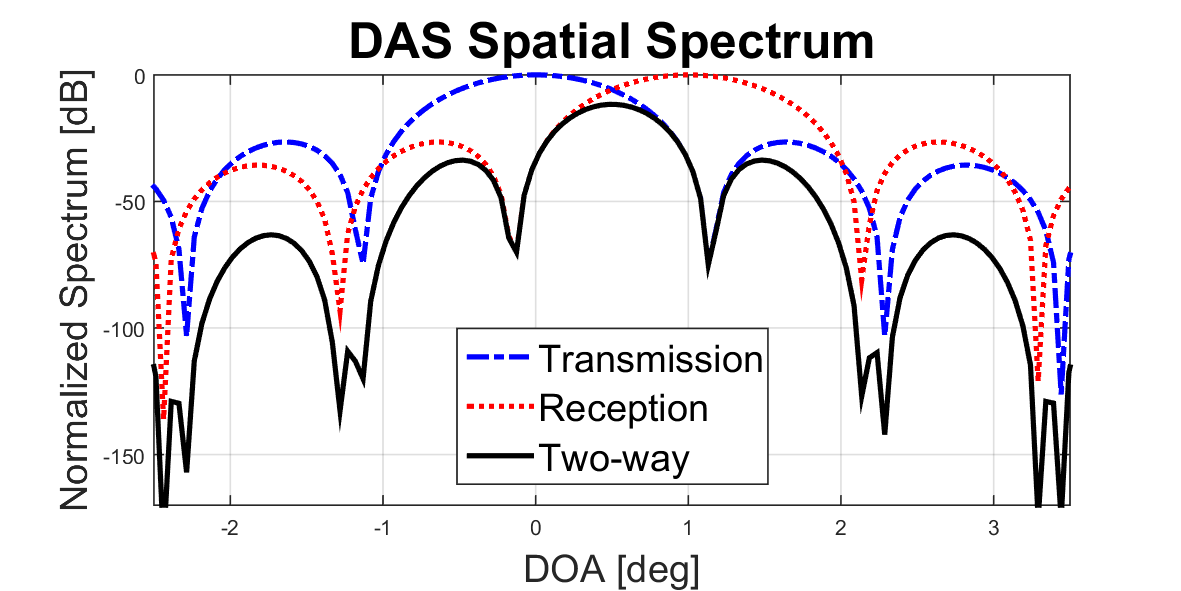
\includegraphics[width=\linewidth]{./images/background/prb.png}
	\caption{Example of DAS transmission, reception and two-way beampatterns with misalignment of transmit and receive beams}
	\label{fig:prb}
\end{figure}

An example of PRB approach is displayed in Figure \ref{fig:prb_3beams}. Three two-way beams are created from a single transmit beam, which means that image acquisition time can be reduced in this case by a factor of three without resolution loss. However, the two-way beams that are not aligned with the transmit beam display lower maximal gain than the one that is aligned.
Their maxima, at -0.5 and $0.5^\circ$ DOA, is also shifted towards that of the transmit beam compared that of their relative receive beams, at -1 and $1^\circ$ DOA.

Several approaches to reducing artifacts caused by PRB exist. Some of them, known as synthetic transmit beams, dynamic steering or the Wright approach, are explained and compared by \cite{prb_approaches}.

\begin{figure}[ht]
    \centering
    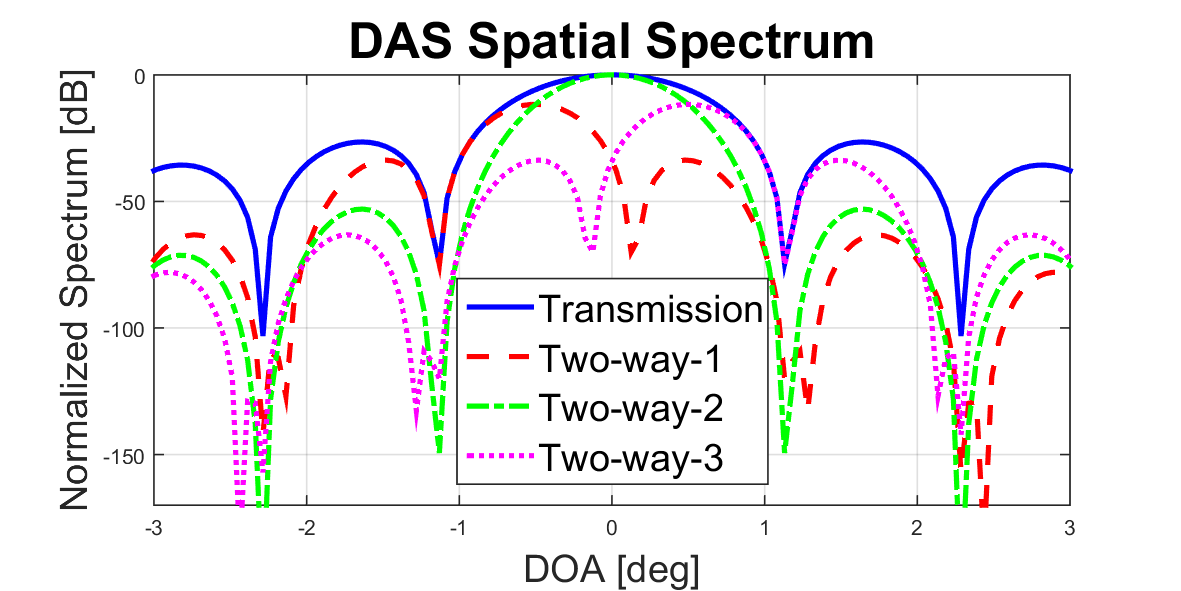
\includegraphics[width=\linewidth]{./images/background/prb_3beams.png}
	\caption{Example of PRB approach, with a single transmit beam centered at $0^\circ$ and 3 receive beams at -1, 0 and $1^\circ$. The resulting two-way beampatterns are displayed along with the transmit beam.}
	\label{fig:prb_3beams}
\end{figure}


\subsection{Covariance matrix estimation}
\label{sec:covariance_estimation}
The covariance matrix of the set of time-delayed recorded signals $\boldsymbol{Y_e}(t)$ is defined $\boldsymbol{R_e}(t) = E[\boldsymbol{Y_e}(t) \boldsymbol{Y_e}^H(t)]$.
Assuming the transducer array to record only monochromatic waves in the far-field (Section \ref{sec:nearfield_farfield}), $\boldsymbol{Y_e}(t)$ can be considered as a \textit{stationary process} in time, which means $\boldsymbol{R_e}$ is only dependent on the focus vector $\boldsymbol{e}$. Considering that all backscatterers in the imaged medium are uncorrelated and $\boldsymbol{Y_e}$ is a stationary process, $\boldsymbol{R_e}$ is a Toeplitz matrix (\cite{van_trees}). A Toeplitz matrix is a matrix whose descending left-to-right diagonals are constants. It notably has the property of being \textit{persymmetric}:
\begin{equation}
    \boldsymbol{R} = \boldsymbol{JR^TJ}, \quad J = \begin{bmatrix}
    0 & 0 & ... & 0 & 1 \\
    0 & 0 & ... & 1 & 0 \\
    : & : & ... & : & : \\
    0 & 1 & ... & 0 & 0 \\
    1 & 0 & ... & 0 & 0
    \end{bmatrix},
\label{eq:persymmetric}
\end{equation}
\noindent
where $\boldsymbol{J}$ is a MxM exchange matrix. This property is notably used by the \textit{forward-backward} approach (Section \ref{sec:fb_averaging}).
\noindent
This matrix is used in Equation (\ref{eq:das_power}) for obtaining the DAS beamformer power output $Z(\boldsymbol{e})$. However, this matrix is unknown and an estimate of it, $\boldsymbol{\tilde{R}(e)}$, needs to be built.

In medical ultrasound imaging, the recorded signals are often broadband and in the array's near field. The assumption that $\boldsymbol{Y}$ is a stationary process is therefore often not true.
However, instead of building a global covariance matrix estimate $\boldsymbol{\tilde{R}}$ for the whole beamformed image, a different covariance matrix estimate $\boldsymbol{\tilde{R}}_{\theta,n}$ can be built for each image sample $Z_{\theta, n}$, i.e each sample range index $n$ and angle index $\theta$.
Note that a range index $n$ can consist of a multiple temporal samples $t$ of the recorded wavefield $\boldsymbol{Y}(t)$ if time averaging (Section \ref{sec:time_averaging}) is used.
The discrete covariance matrix estimate $\boldsymbol{\tilde{R}}_{\theta,n}$ can be expressed as follow:
\begin{equation}
    \tilde{\boldsymbol{R}}_{\theta,n} = \frac{1}{2T+1} \sum_{t=-T}^{T} \boldsymbol{Y_e}[n - t] \boldsymbol{Y_e}^H[n - t],
\label{eq:cov_matrix}
\end{equation}
\noindent
where $2T + 1$ is the number of temporal samples per radial range and $\boldsymbol{Y_e}$ is the set of recorded wavefield time-shifted by vector $\boldsymbol{e}$. The time-delay focus vector $\boldsymbol{e}$ can be defined as a function of $n$ and $\theta$.
The local estimates of $\boldsymbol{R_e}$ should then technically be defined as $\boldsymbol{\tilde{R}}_{\boldsymbol{e}(\theta,n)}$.
We have chosen to simplify the notation to $\tilde{\boldsymbol{R}}_{\theta,n}$.

Yet, even for local estimates of $\boldsymbol{R_e}$, $\boldsymbol{Y_e}$ is not always stationary. In medical ultrasound imaging, it is often the case that the transducer array is sending short pulses and only recording a few temporal samples $t$ per radial range $n$. This means that the pulse reflected by a target out of the array's focus might not be recorded by all transducers for the same sample range $n$. However, the stationary assumption holds for targets close to the array's focus point, since the recorded data is aligned such that their reflected signal adds up coherently.